\documentclass{article}
\usepackage[utf8]{inputenc}
\usepackage{graphicx}
\usepackage{subcaption}
\usepackage{amsmath}

\title{Image and Video Processing Lab 2}
\author{Philine Witzig}
\date{October 2020}

\begin{document}

\maketitle
General notes: when running the matlab script, you will be asked to enter the number of the task you want to test. Enter the numbers $1$ to $7$ in order to test the respective task. All subtasks will be executed. In Section \ref{sec:discussion}, you can find Table \ref{tab:1} as a support for the arguments made in the discussion paragraph of each section.
\section{Fixed Threshold Method}
To implement the fixed threshold method, the matlab function \textsf{imbinarize(I, t)} was used. It converts the grayscale image \textsf{I} to a binary image, by replacing all pixels in the input image with luminance greater than the passed threshold level \textsf{t} with the value 1 (white) and replacing all other pixels with the value 0 (black). \textsf{t} was chosen to be half the dynamic range of \textsf{I}, normalized to be in range $[0, 1]$. Figure \ref{fig:fixed_thresh} visualizes the fixed threshold results for, both, \textsf{lena-y.png} and \textsf{wool.png}.

  \begin{figure}
        \centering
        \begin{subfigure}[b]{0.49\textwidth}
            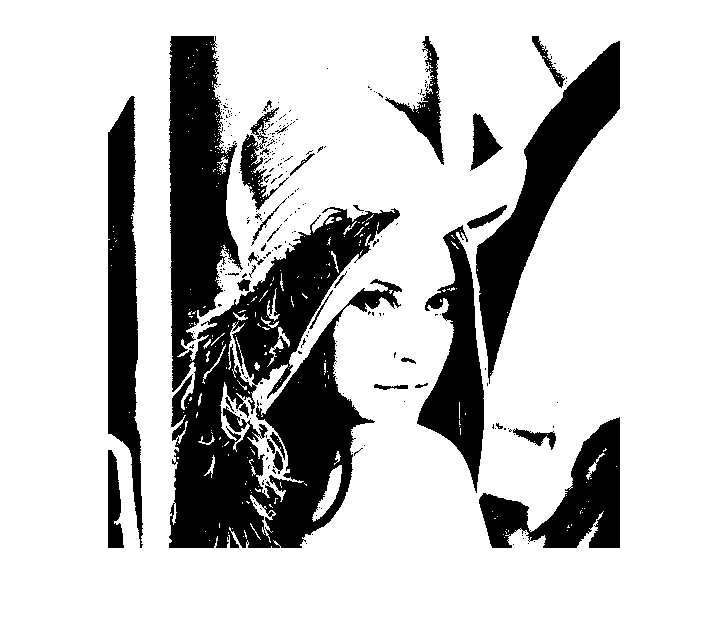
\includegraphics[width=\textwidth]{Images/lena_fixed_thresh.png}
            \subcaption{$\textsf{t} = 0.43529$}
        \end{subfigure}
        \begin{subfigure}[b]{0.49\textwidth}
            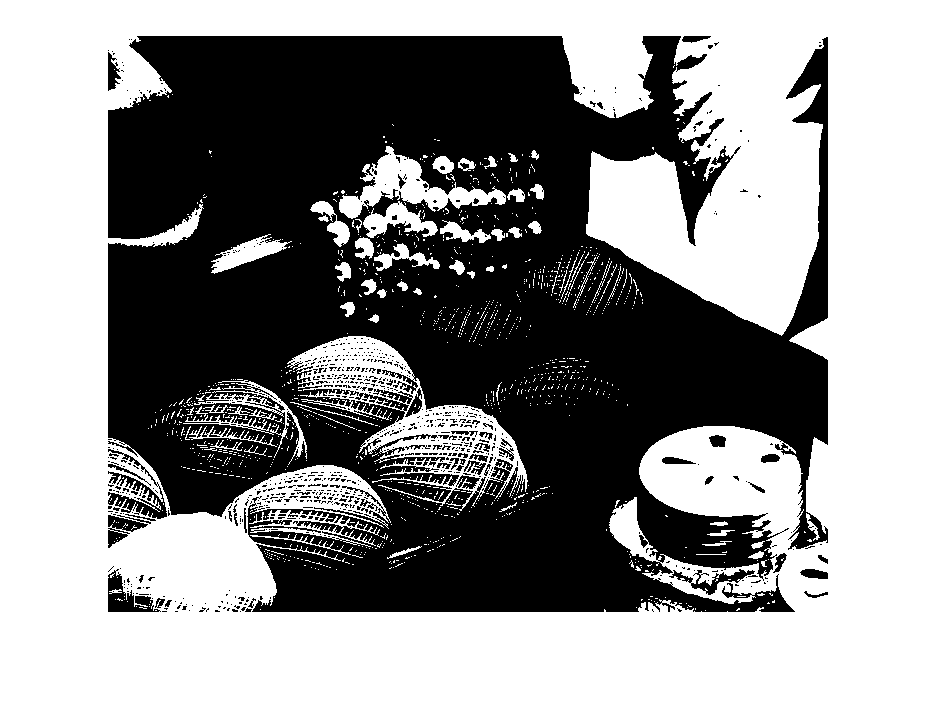
\includegraphics[width=\textwidth]{Images/wool_fixed_thresh.png}
            \subcaption{$\textsf{t} = 0.47059$}
        \end{subfigure}
        \caption{Fixed threshold method on \textsf{lena-y.png} and \textsf{wool.png}.}
        \label{fig:fixed_thresh}
    \end{figure}
    
\paragraph{Discussion} What we can clearly observe in Figure \ref{fig:fixed_thresh} is that we do not obtain visually good results using the fixed threshold method since we loose most of the shade information and details (e.g. confer shoulder region, does not appear curved anymore). However, this method is the fastest. Although it visually produces the worst results, it interestingly has a comparably small MSE (cf. Table \ref{tab:1}). 

\section{Random Threshold Method}
For this exercise, uniform random noise was created using matlab's \textsf{unidrnd(n, height, width)} function. The noise amplitude can be set by passing a coefficient between $0$ and $1$ to the \textsf{random\_threshold(I, coeff)} method. Once the noise is added to the input image, it is thresholded as before. The noise amplitudes were estimated empirically in such a way that they would best reproduce the original image (cf. Figure \ref{fig:rand_thresh}).
 \begin{figure}
        \centering
        \begin{subfigure}[b]{0.49\textwidth}
            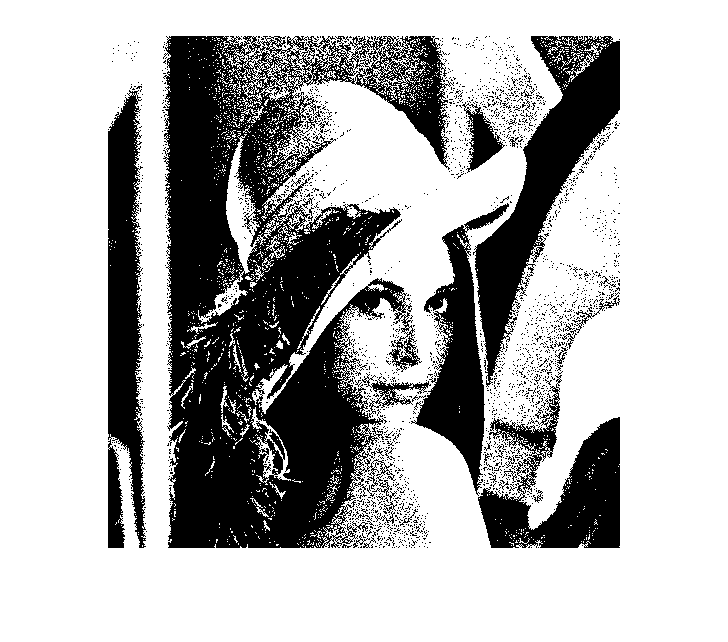
\includegraphics[width=\textwidth]{Images/lena_rand_thresh.png}
            \subcaption{Noise amplitude: $0.2$}
        \end{subfigure}
        \begin{subfigure}[b]{0.49\textwidth}
            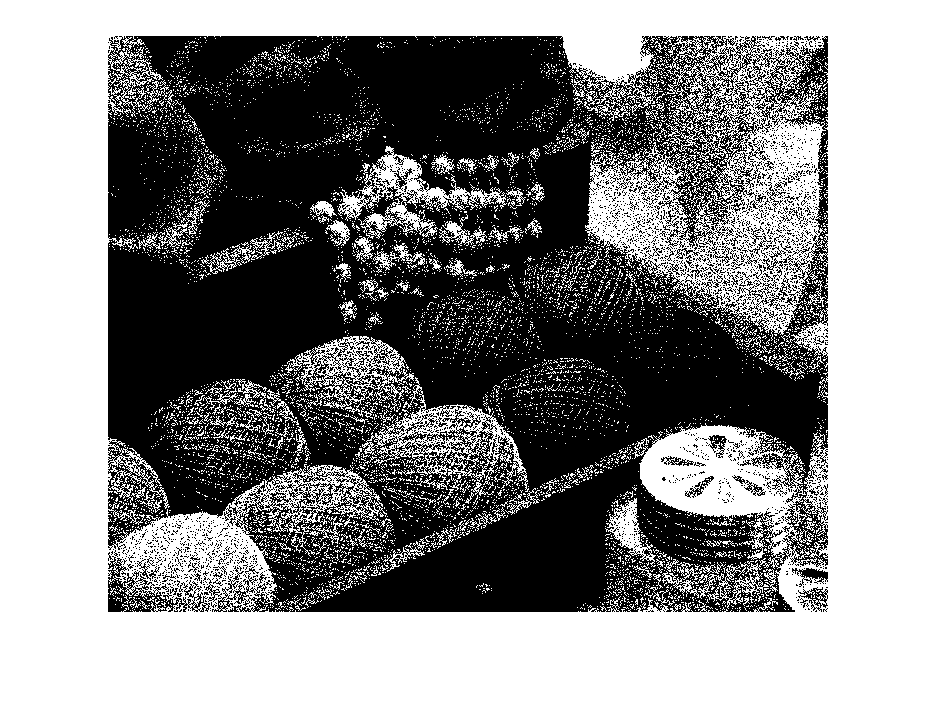
\includegraphics[width=\textwidth]{Images/wool_rnd_thresh.png}
            \subcaption{Noise amplitude: $0.6$}
        \end{subfigure}
        \caption{Random threshold method on \textsf{lena-y.png} and \textsf{wool.png} with different amplitudes for noise.}
        \label{fig:rand_thresh}
\end{figure}

\paragraph{Discussion}
Compared to the fixed threshold method, the random threshold method is able to compensate for the extreme loss in detail and is capable of capturing gray levels. It is interesting, however, that it not necessarily leads to an improvement in the MSE. Furthermore, if we zoom into the image, we observe the noise becomes more prominent and sharp edges become cracked.

\section{Ordered Threshold Method}
For this exercise, the quantization operator and the ordered threshold method had to be implemented. The \textsf{quantize(I, lower, upper)} takes as arguments the input image which is to be quantized as well as an upper bound $u$ and a lower bound $l$. The quantization $v'$ of a pixel $v$ is then computed as follows:
\begin{equation*}
    v' = \frac{(v - v_{min}) \cdot (u - l)}{(v_{max} - v_{min}) + l},
\end{equation*}
where $v_{min}$ is the minimal pixel value and $v_{max}$ is the maximum pixel value in the input image. The \textsf{ordered\_thresh(I, M)} method now takes the quantized image \textsf{I} and moves the threshold mask \textsf{M} over the image. For each pixel in \textsf{I}, we check if its value is smaller than the corresponding pixel at the same position in \textsf{M}. If this is the case, it is set to $0$, otherwise $1$. This operation is realized through a one-line \textsf{if-else} statement, i.e.
\begin{equation*}
    (a > b) \cdot c + (\neg(a > b)) \cdot d,
\end{equation*}
where $a$ is the value of the current pixel in \textsf{I}, $b$ is the value of the corresponding pixel in \textsf{M}, $c$ is $1$ and $d$ is $0$.
\section{Ordered Matrix with Centered Points}
We now applied the above functions to the input images using different masks, i.e. $C_6$ creating ``central central white points over a black background" and $E_6$ called ``balanced centered points". The respective results can be seen in Figure \ref{fig:ordered_thresh_lena} and Figure \ref{fig:ordered_thresh_wool}. 
 \begin{figure}
        \centering
        \begin{subfigure}[b]{0.49\textwidth}
            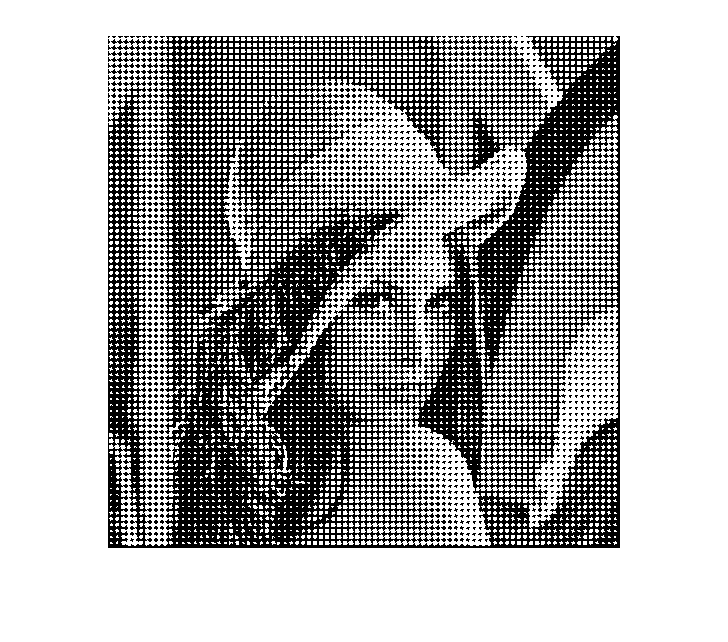
\includegraphics[width=\textwidth]{Images/lena_ordered_c6.png}
            \subcaption{Central white points ($C_6$)}
        \end{subfigure}
        \begin{subfigure}[b]{0.49\textwidth}
            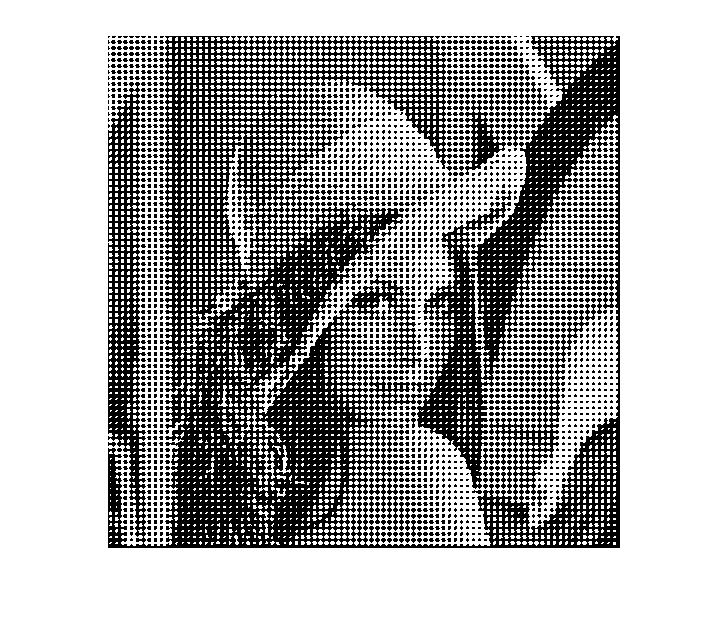
\includegraphics[width=\textwidth]{Images/lena_ordered_e6.png}
            \subcaption{Balanced white points ($E_6$)}
        \end{subfigure}
        \caption{Ordered threshold method on \textsf{lena-y.png} with different masks.}
        \label{fig:ordered_thresh_lena}
\end{figure}

 \begin{figure}
        \centering
        \begin{subfigure}[b]{0.49\textwidth}
            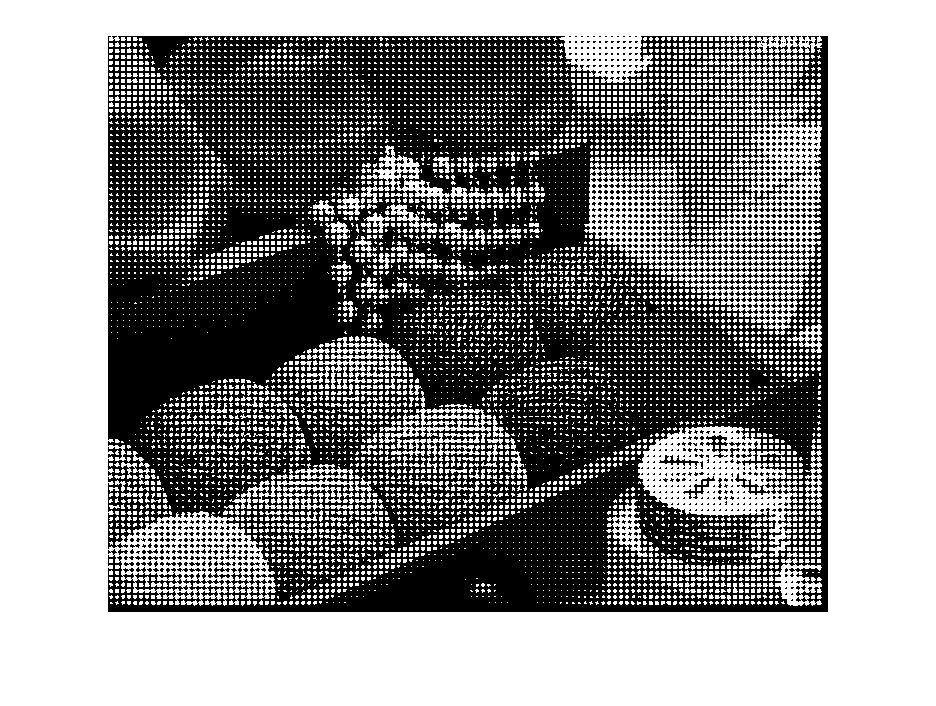
\includegraphics[width=\textwidth]{Images/wool_ordered_c6.png}
            \subcaption{Central white points ($C_6$)}
        \end{subfigure}
        \begin{subfigure}[b]{0.49\textwidth}
            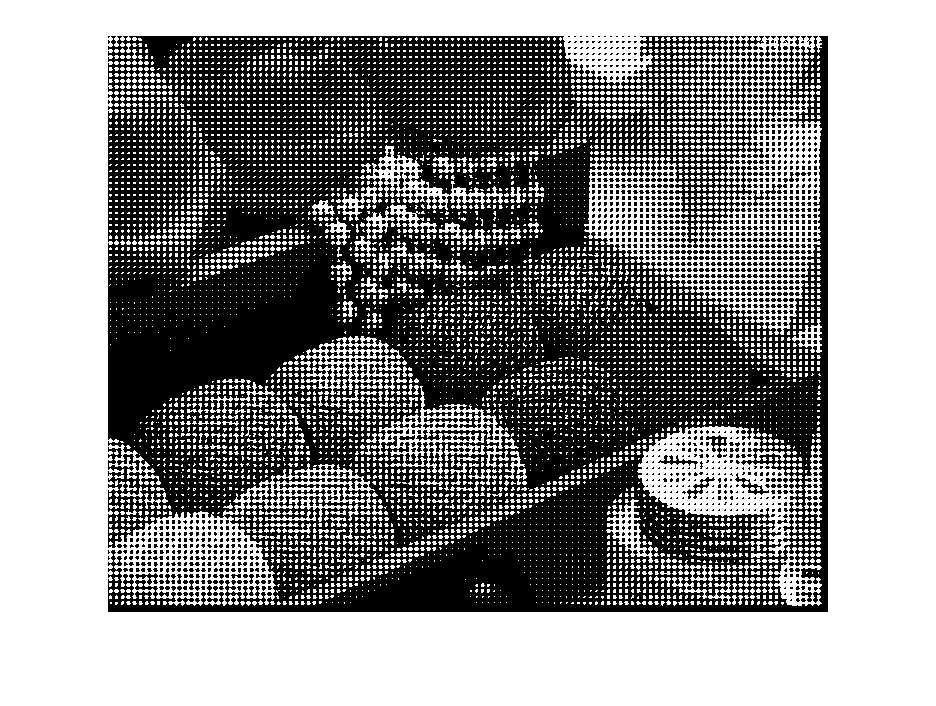
\includegraphics[width=\textwidth]{Images/wool_ordered_e6.png}
            \subcaption{Balanced white points ($E_6$)}
        \end{subfigure}
        \caption{Ordered threshold method on \textsf{wool.png} with different masks.}
        \label{fig:ordered_thresh_wool}
\end{figure}
\paragraph{Discussion} The first thing which is observable is that the method as implemented here produces boundary artifacts if the \textsf{I}'s size is not an exact multiple of \textsf{M}' size. Secondly, both masks produce white dots on a black ground/ black dots on a white ground which are highly aligned to the horizontal and the vertical axis. This grid pattern becomes visible in the dithered version. However, the main difference between the two masks can be observed in the shape of the points where $E_6$ seems to produce more round dots.
Furthermore, $E_6$ seems to be a little faster compared to $C_6$.

\section{Diagonal Ordered Matrix with Balanced Centered Points}
For the diagonal ordered matrix, the results shown in Figure \ref{fig:diagonal_ordered} were obtained. 
 \begin{figure}
        \centering
        \begin{subfigure}[b]{0.49\textwidth}
            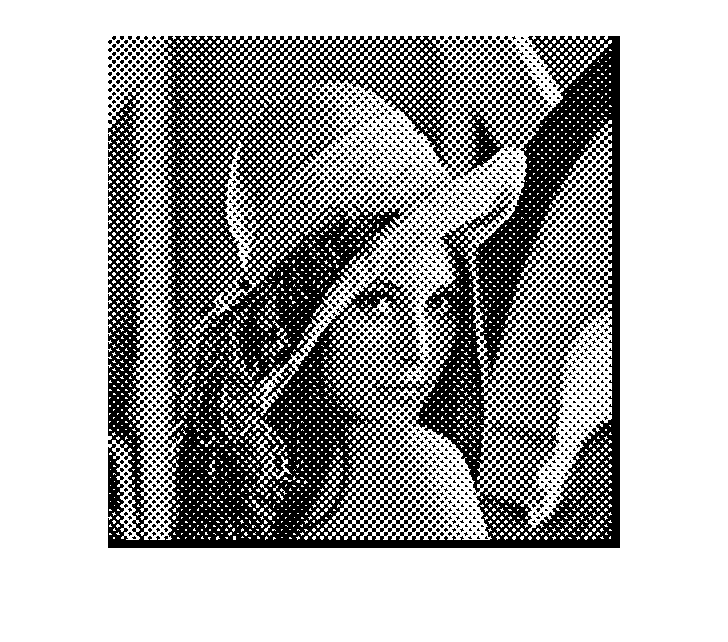
\includegraphics[width=\textwidth]{Images/lena_diagonal_ordered.png}
            \subcaption{\textsf{lena-y.png}}
        \end{subfigure}
        \begin{subfigure}[b]{0.49\textwidth}
            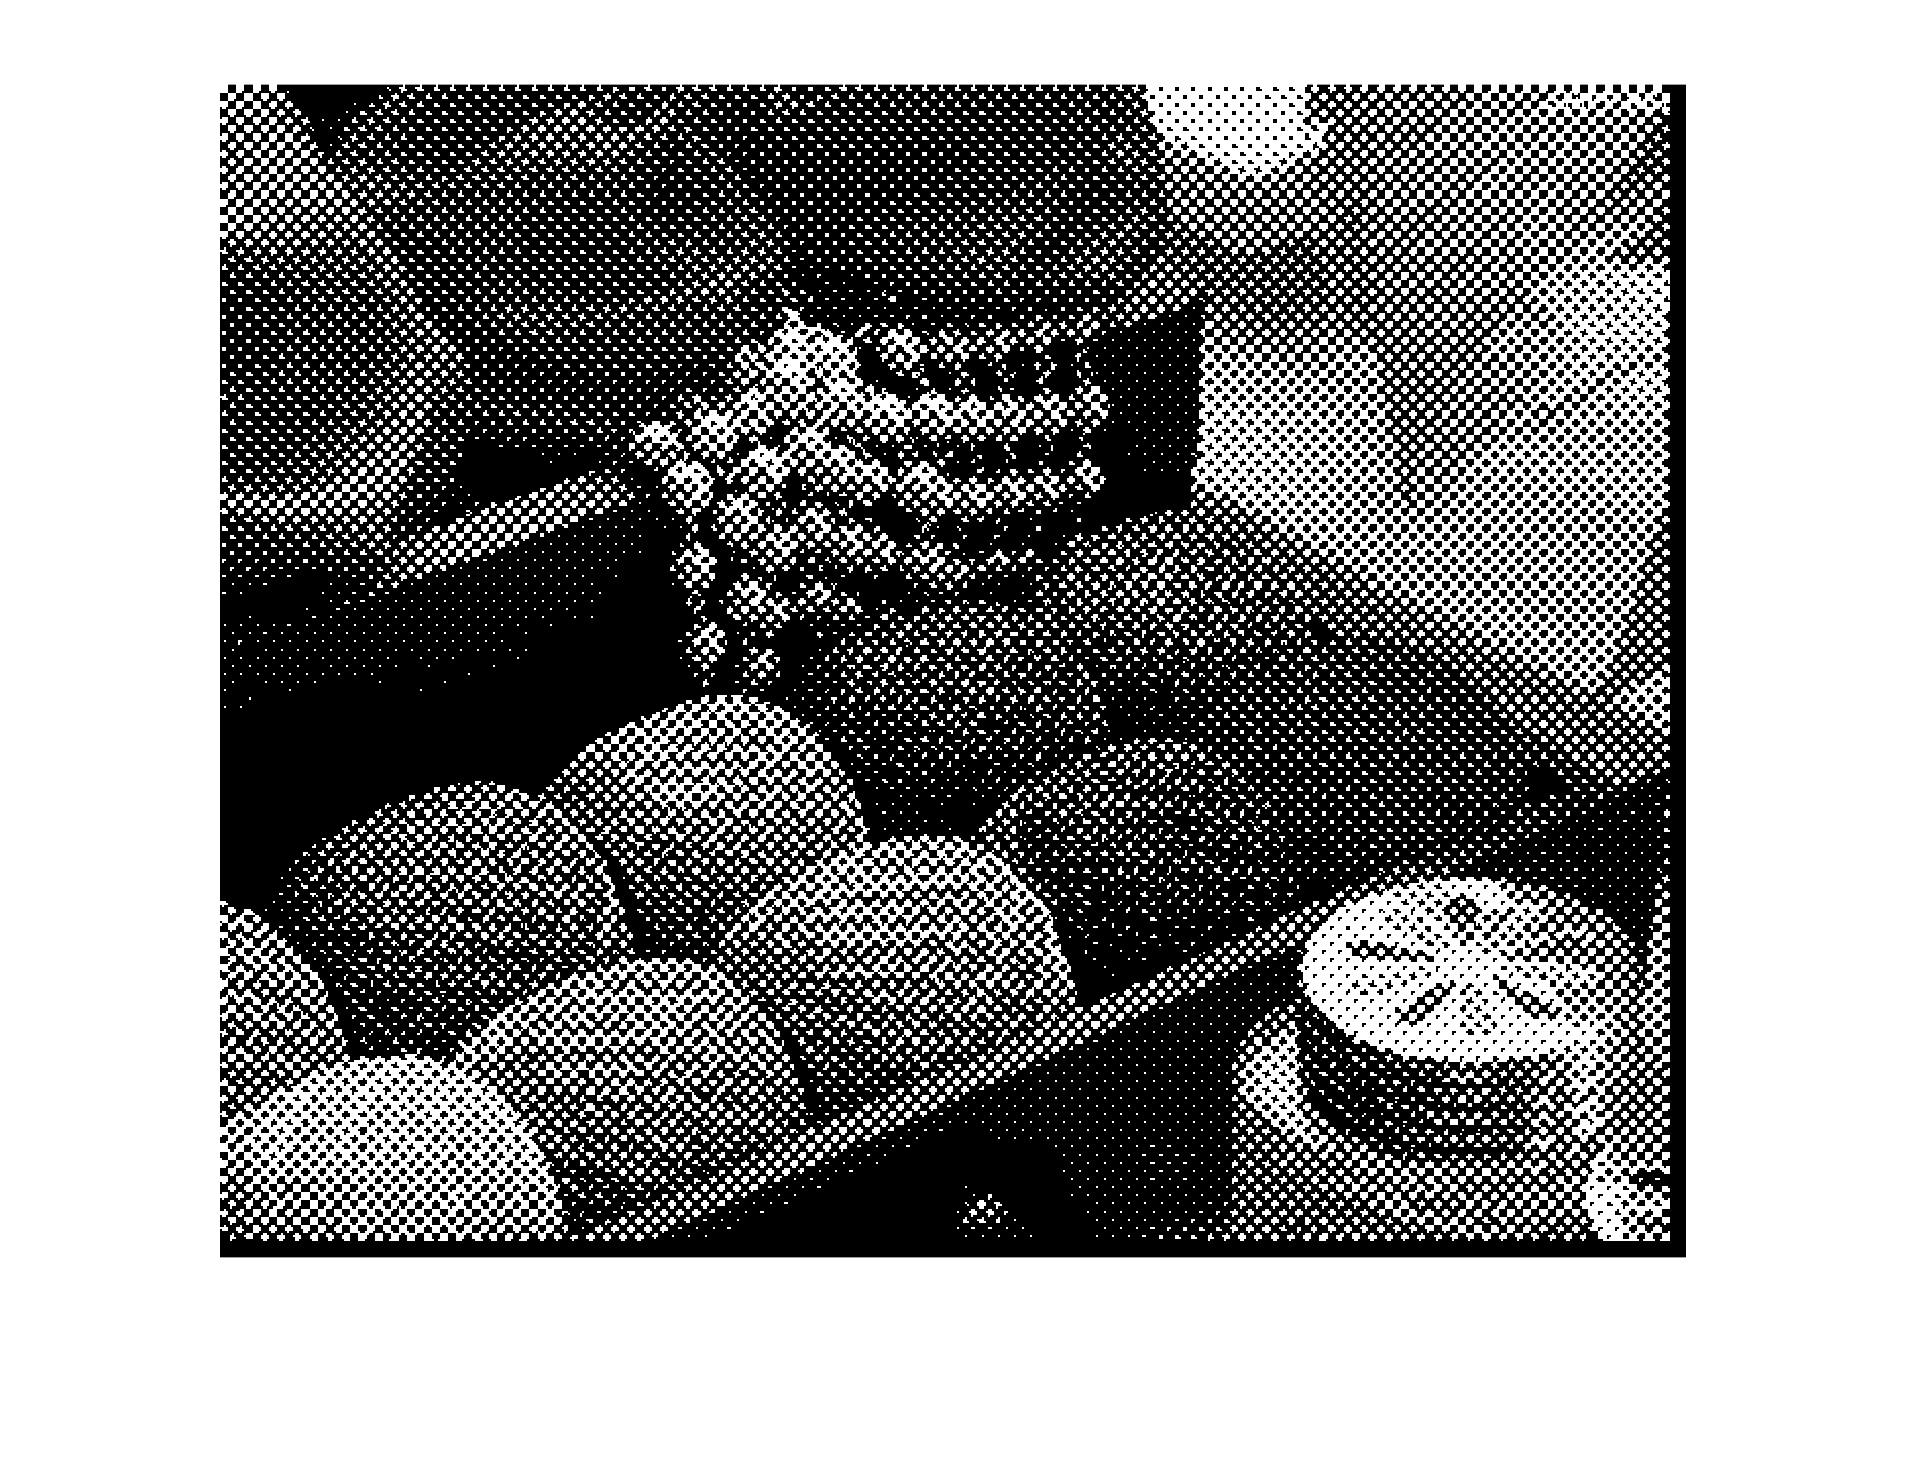
\includegraphics[width=\textwidth]{Images/wool_diagonal_ordered.png}
            \subcaption{\textsf{wool.png}}
        \end{subfigure}
        \caption{Ordered threshold method with diagonal filter element.}
        \label{fig:diagonal_ordered}
\end{figure}
\paragraph{Discussion} We can observe that with the diagonal ordered mask, the axis aligned patterns which were visible in the previous task are a lot less dominant. If we zoom in on the results, we can see that as suggested by the exercise description we also obtain diagonal dots. Thus, it can be assumed that the human visual system is a lot more sensitive to horizontal and vertical patterns than to diagonal patterns. 

\section{Ordered Matrix with Dispersed Dots}
For the ordered method with dispersed dots, we obtain the result shown in Figure \ref{fig:diagonal_dispersed}.
 \begin{figure}
        \centering
        \begin{subfigure}[b]{0.49\textwidth}
            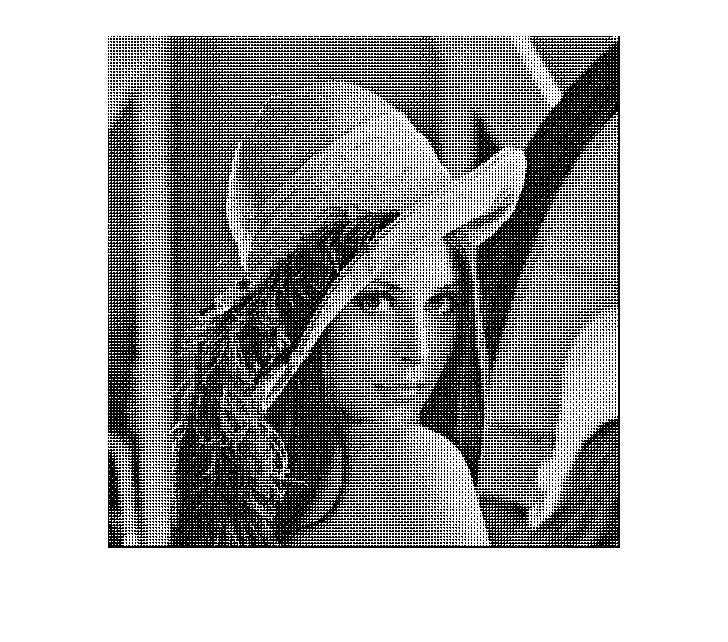
\includegraphics[width=\textwidth]{Images/lena_diagonal_dispersed.png}
            \subcaption{\textsf{lena-y.png}}
        \end{subfigure}
        \begin{subfigure}[b]{0.49\textwidth}
            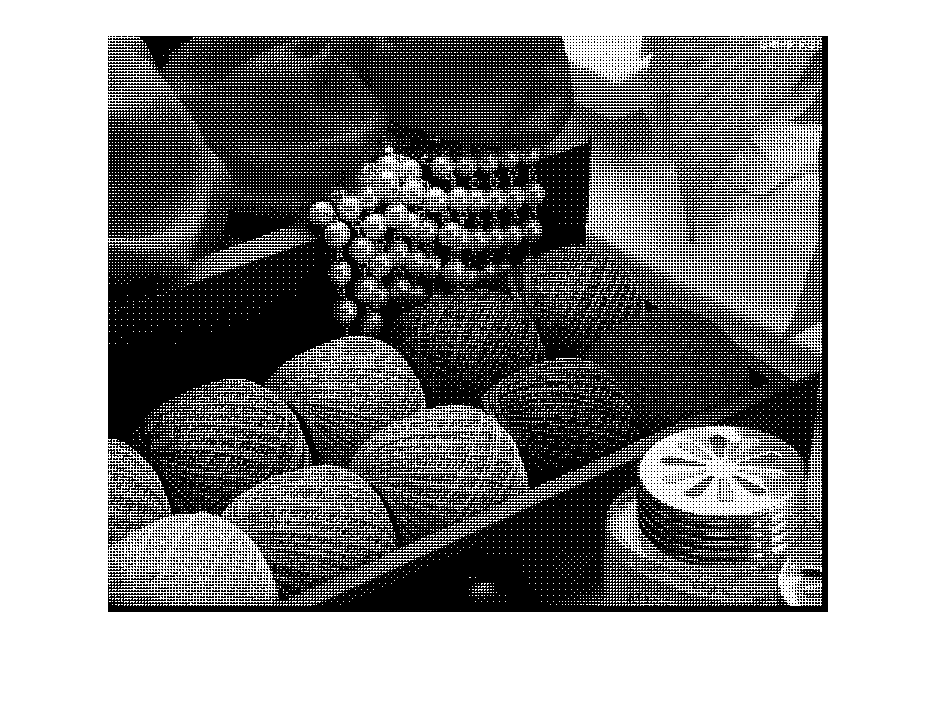
\includegraphics[width=\textwidth]{Images/wool_dispersed.png}
            \subcaption{\textsf{wool.png}}
        \end{subfigure}
        \caption{Ordered threshold method with Bayer's mask.}
        \label{fig:diagonal_dispersed}
\end{figure}
\paragraph{Discussion} Applying Bayer's pattern using the ordered threshold method leads to the presence of cross-hatch patterns. Especially dark areas are completely colored in black without any dots available (cf. \textsf{wool.png} back box). Again, horizontal and vertical patterns are visible just like in Exercise 4.
\section{Error Diffusion Method}
For the error diffusion method, we aim at distributing the dithering error to neighboring pixels. Fot this, a threshold \textsf{t} was computed using the dynamic range of the input image as before and the input image \textsf{I} was scaled to range from $0$ to $1$ using matlab's \textsf{rescale(I)} method. It scales the entries of an \textsf{I} to the interval [0,1]. The custom \textsf{error\_diffusion(I, filter, t)} method then realizes the actual error distribution. For each \textsf{I}$(y, x) = v$, it computes its binary value $v'$ using \textsf{t}, sets $\textsf{I}(y, x) = v'$ and computes the intensity error $e = v - v'$. The error is then distributed to the neighboring pixels based on some filter pattern, which is implemented as an array with format $(y_{\text{off}}, x_{\text{off}}, c)$, where $y_{\text{off}}$ and $x_{\text{off}}$ are the offsets from pixel $(y, x)$ with value $v$ and $c = \textsf{filter}(y + y_{\text{off}}, x + x_{\text{off}})$. Putting this into one equation, this yields:
\begin{equation*}
    \textsf{I}(y + y_{\text{offset}}, x_{\textsf{off}}) = \textsf{I}(y + y_{\text{off}}, x + x_{\text{off}}) + \textsf{filter}(y + y_{\text{off}}, x + x_{\text{off}}) \cdot e.
\end{equation*}

\begin{figure}
        \centering
        \begin{subfigure}[b]{0.49\textwidth}
            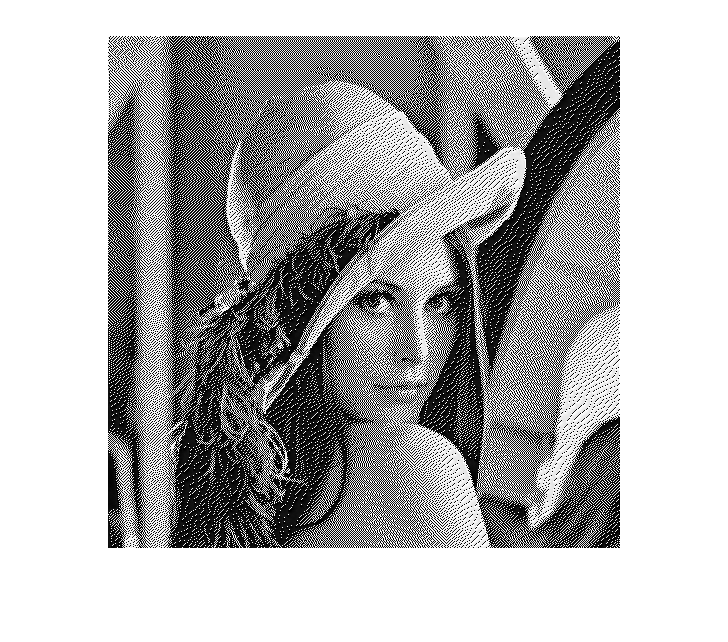
\includegraphics[width=\textwidth]{Images/lena_error_diffusion_floyd.png}
            \subcaption{Floyd \& Steinberg filter}
        \end{subfigure}
        \begin{subfigure}[b]{0.49\textwidth}
            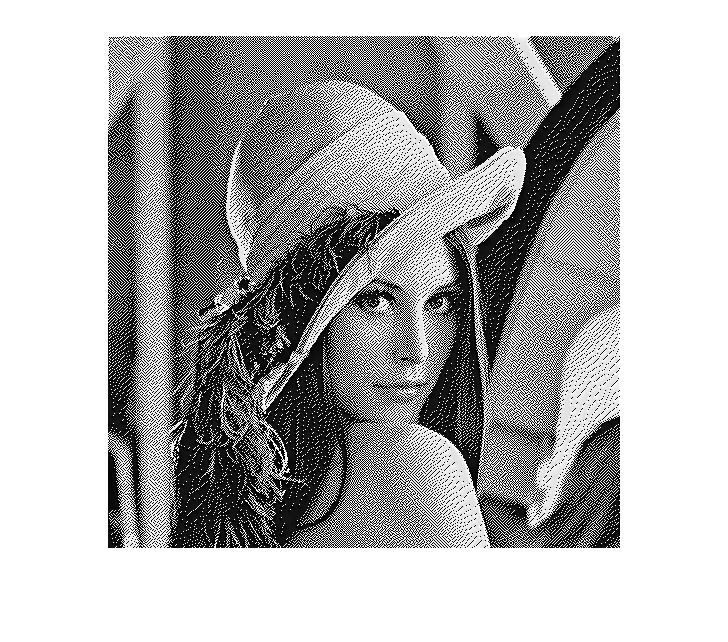
\includegraphics[width=\textwidth]{Images/lena_error_diffusion_stucki.png}
            \subcaption{Stucki filter}
        \end{subfigure}
        \caption{Error diffusion method on \textsf{lena-y.png} using different filters.}
        \label{fig:error_diff_lena}
\end{figure}

\begin{figure}
        \centering
        \begin{subfigure}[b]{0.49\textwidth}
            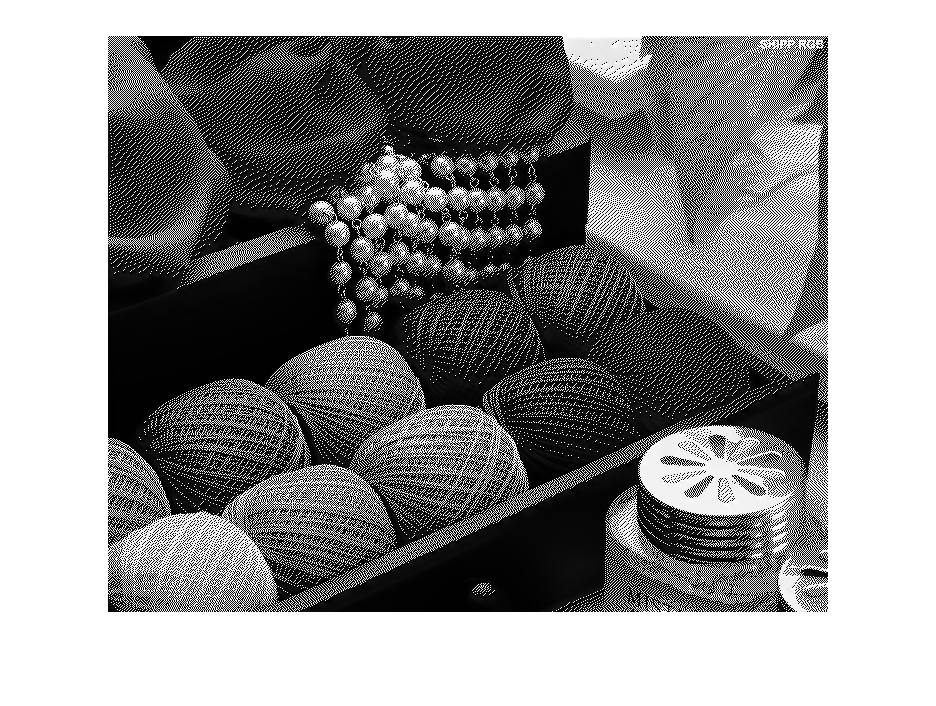
\includegraphics[width=\textwidth]{Images/wool_error_diffusion_floyd.png}
            \subcaption{Floyd \& Steinberg filter}
        \end{subfigure}
        \begin{subfigure}[b]{0.49\textwidth}
            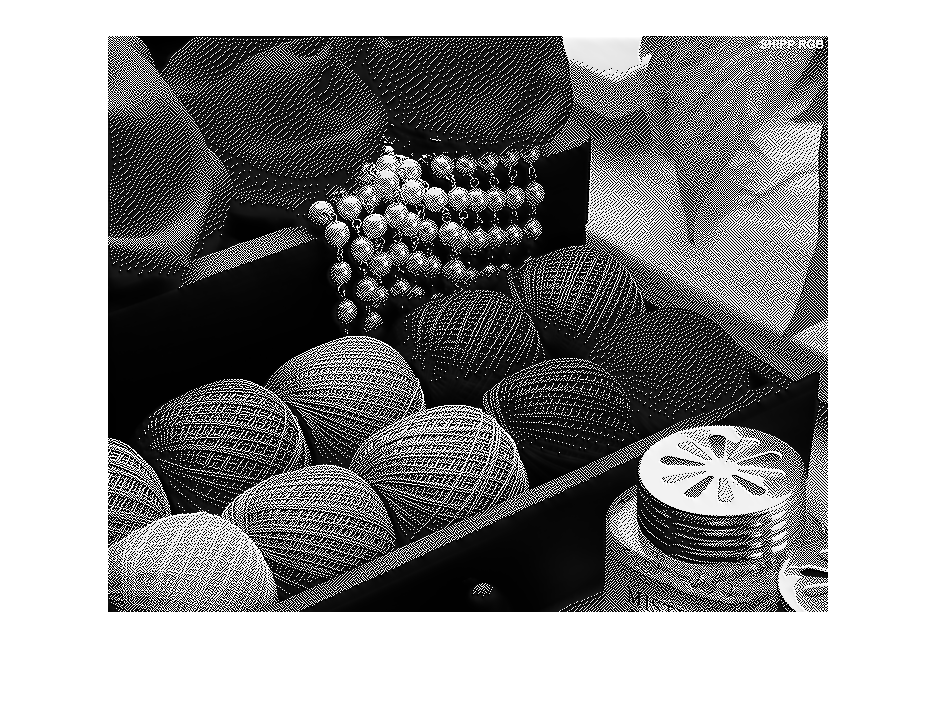
\includegraphics[width=\textwidth]{Images/wool_error_diffusion_stucki.png}
            \subcaption{Stucki filter}
        \end{subfigure}
        \caption{Error diffusion method on \textsf{wool.png} using different filters.}
        \label{fig:error_diff_wool}
\end{figure}
\paragraph{Discussion} Comparing the results in Figure \ref{fig:error_diff_lena} and Figure \ref{fig:error_diff_wool}, we can clearly say that the error diffusion method produces the visually best results. For \textsf{wool.png}, even the letters on the box at the bottom and at the top right corner remain visible. Edges remain sharp and details are sufficiently preserved. Comparing the Floyd \& Steinberg filter to the Stucki filter, one can say that Floyd \& Steinberg results in a very fine-grained dithering since it diffuses the error only to the immediate neighboring pixels. Stucki's dithering, in contrast, is a little coarser as it also considers second-level neighbors (i.e. not only the immediate neighbors). As expected, it has a larger computation time since it considers a larger neighborhood. Last but not least, Stucki's filter produces a smaller MSE compared to Floyd \& Steinberg.

\section{Discussion}\label{sec:discussion}
In Table \ref{tab:1}, you can find a final comparison of the dithering methods described above considering visual quality, mean-square error and complexity. Overall, one can say that we obtain the visually best results using the error diffusion methods. The ordered threshold methods all produce comparable results in terms of MSE and only differ amongst each other in terms of complexity and whether a grid pattern is perceived or not. The fastest method is the fixed threshold method. However, we obtain the visually poorest results. Finally, it is important to mention that a \textit{low MSE} does \textit{not} necessarily mean we obtain \textit{visually good} results.
\begin{table}
\centering
\caption{Comparison of dithering methods, results as (\textsf{lena-y.png}, \textsf{wool.png}).}
\begin{tabular}{ c || c | c | c}
 Method & MSE & Complexity in $ms$& Visual results \\ 
 \hline
 Fixed Thresh & (0.134, 0.089) & (2.180, 0.936) & large detail loss\\  
 Random Thresh & (0.126, 0.115) & (16.251, 13.992) & noisy, cracked edges \\ 
 Ordered Thresh C6 & (0.202, 0.157) & (21.592, 8.038) & grid pattern \\ 
 Ordered Thresh E6 & (0.203, 0.157) & (10.635, 7.405) & grid pattern \\ 
 Ordered Thresh O8 & (0.204, 0.157) & (22.924, 13.324) & diagonal blobs, no grid \\
 Ordered Thresh D6 & (0.202, 0.157) & (22.615, 11.349) & grid pattern \\  
 Error diffusion F\&S & (0.181, 0.138) & (69.051, 66.876) & best, fine dithering \\ 
 Error diffusion Stucki& (0.172, 0.128) & (120.385, 176.763) & best, coarser dithering 
\end{tabular}
\label{tab:1}
\end{table}
\end{document}
